\chapter{Proceso de instalación}

El lenguaje NoSQL que hemos escogido para el desarrollo de este trabajo es MongoDB, más particularmente su servicio Atlas: un clúster en la nube que, aun con alternativas de pago, nos permite trabajar los contenidos de este trabajo sin limitaciones.
Lo primero es registrarnos: tras introducir nuestros datos personales, tendremos que seleccionar algunas opciones para nuestro clúster, entre ellas el servidor que nos va a hostear, la región de este, o elegir un plan de pago según nuestras necesidades.

\begin{figure}[!h]
  \centering
    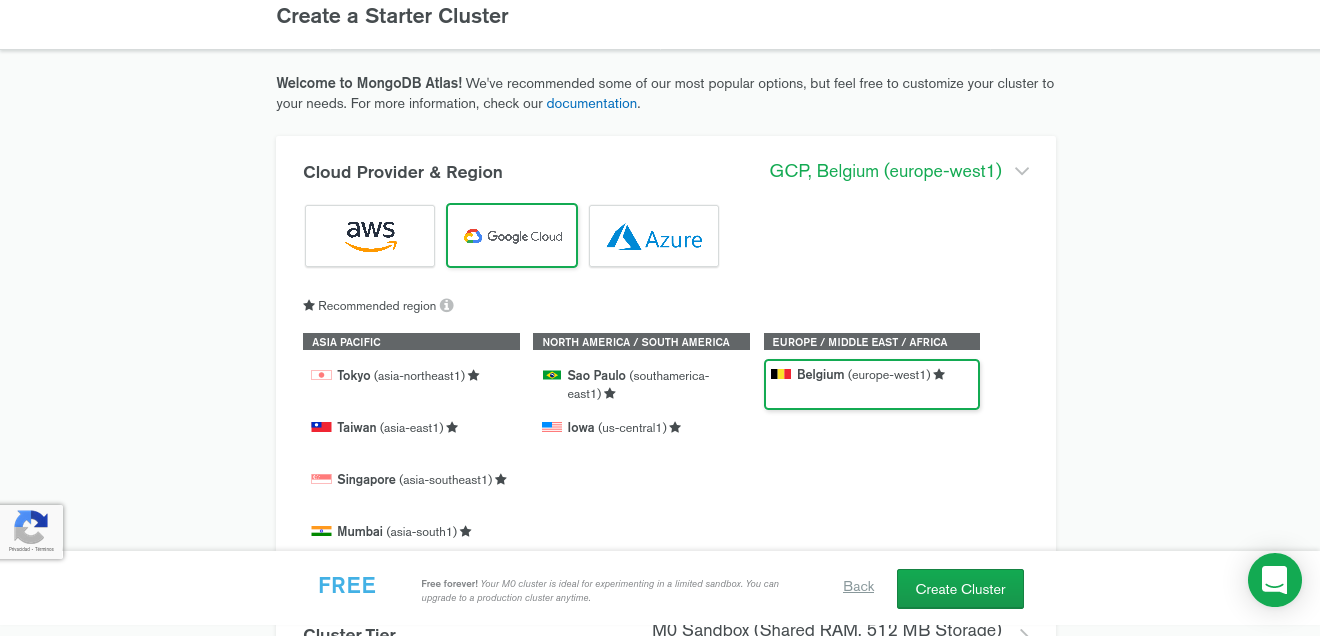
\includegraphics[scale=0.35]{1.png}
\end{figure}

\begin{figure}[!h]
  \centering
    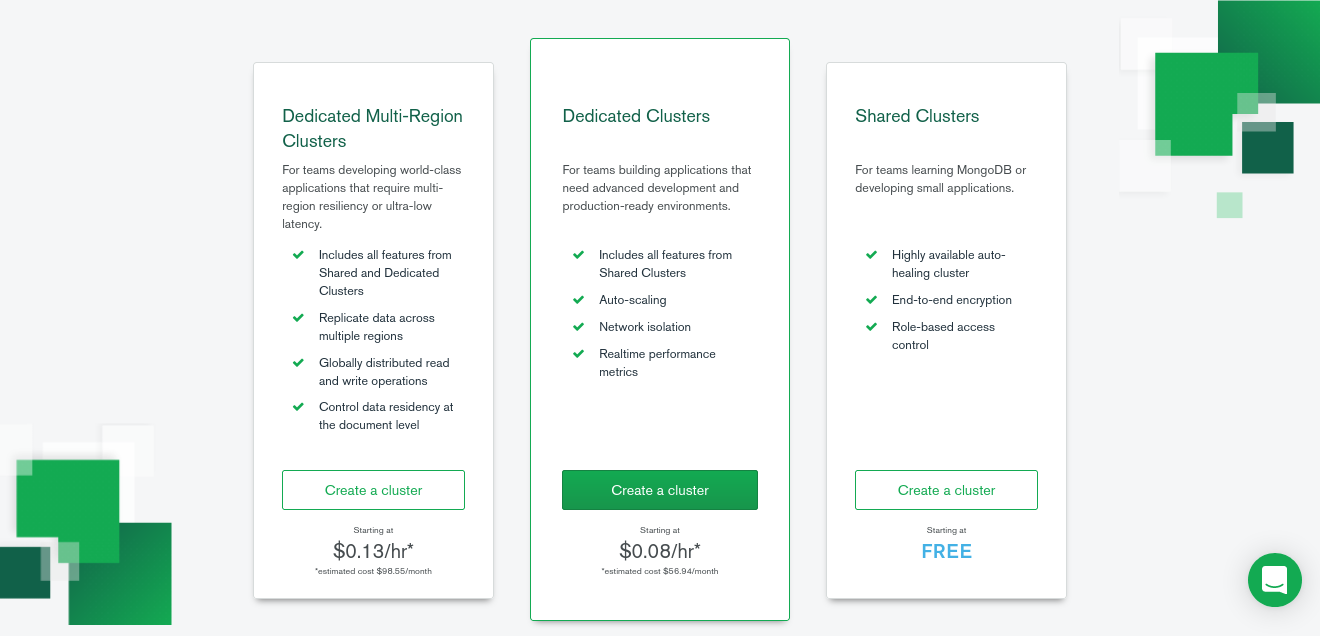
\includegraphics[scale=0.35]{2.png}
\end{figure}

\pagebreak
Para este trabajo hemos escogido las opciones gratuítas: clúster compartido, y un servidor de Google Cloud en Bélgica. Una vez confirmemos la configuración, se creará nuestro clúster. Esto tomará algo menos de 5 minutos.

\begin{figure}[!h]
  \centering
    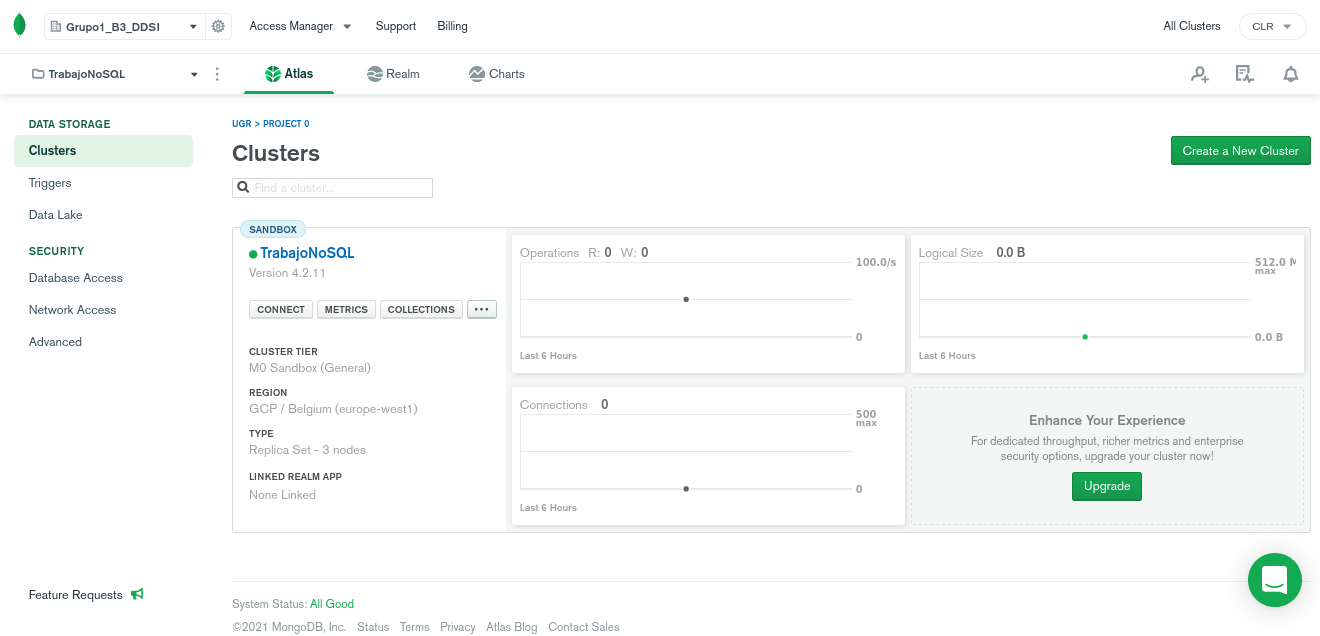
\includegraphics[scale=0.4]{3.png}
\end{figure}

Una vez desplegado el clúster, tenemos que conectarnos. Desde el botón Connect añadiremos nuestra dirección IP. También crearemos un usuario: si somos el primer user, recibiremos por defecto permisos de administrador Atlas.

\begin{figure}[!h]
  \centering
    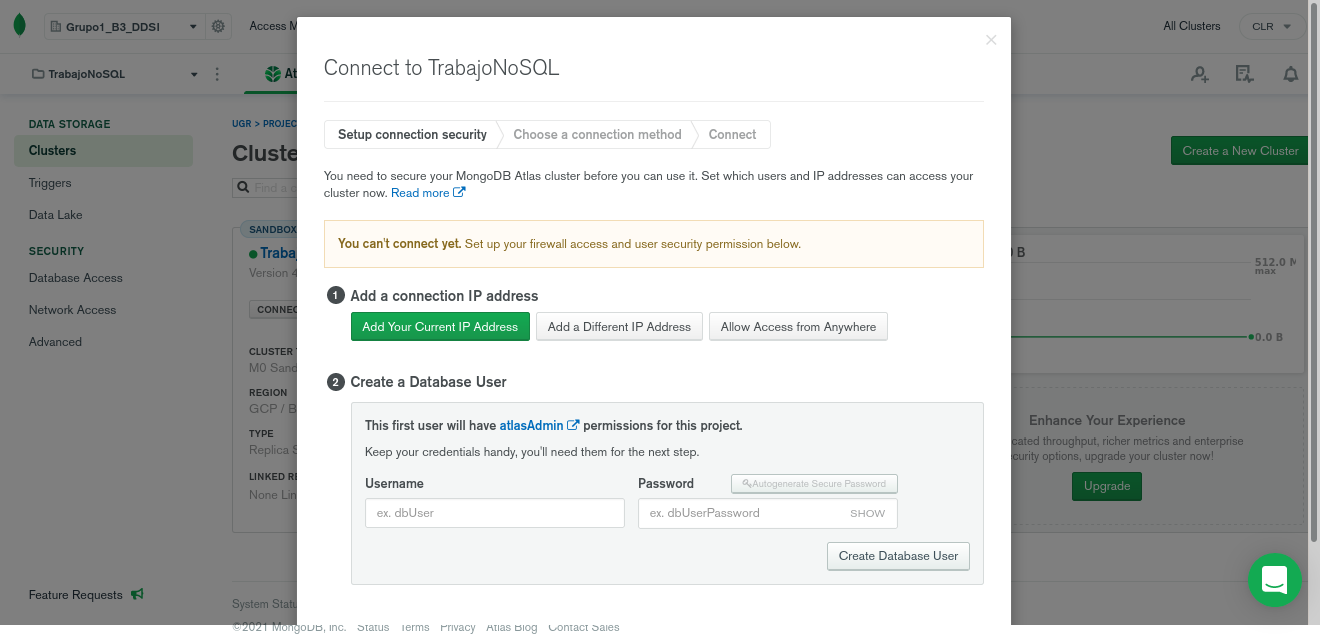
\includegraphics[scale=0.4]{4.png}
\end{figure}

\pagebreak
A continuación escogemos como nos vamos a conectar al clúster: las opciones son la shell de mongoDB (y ejecutar desde la terminal), seleccionar un driver para aplicaciones en python o javascript, y su GUI, MongoDB Compass. Para facilitar el desarrollo de este trabajo hemos escogido Compass.

\begin{figure}[!h]
  \centering
    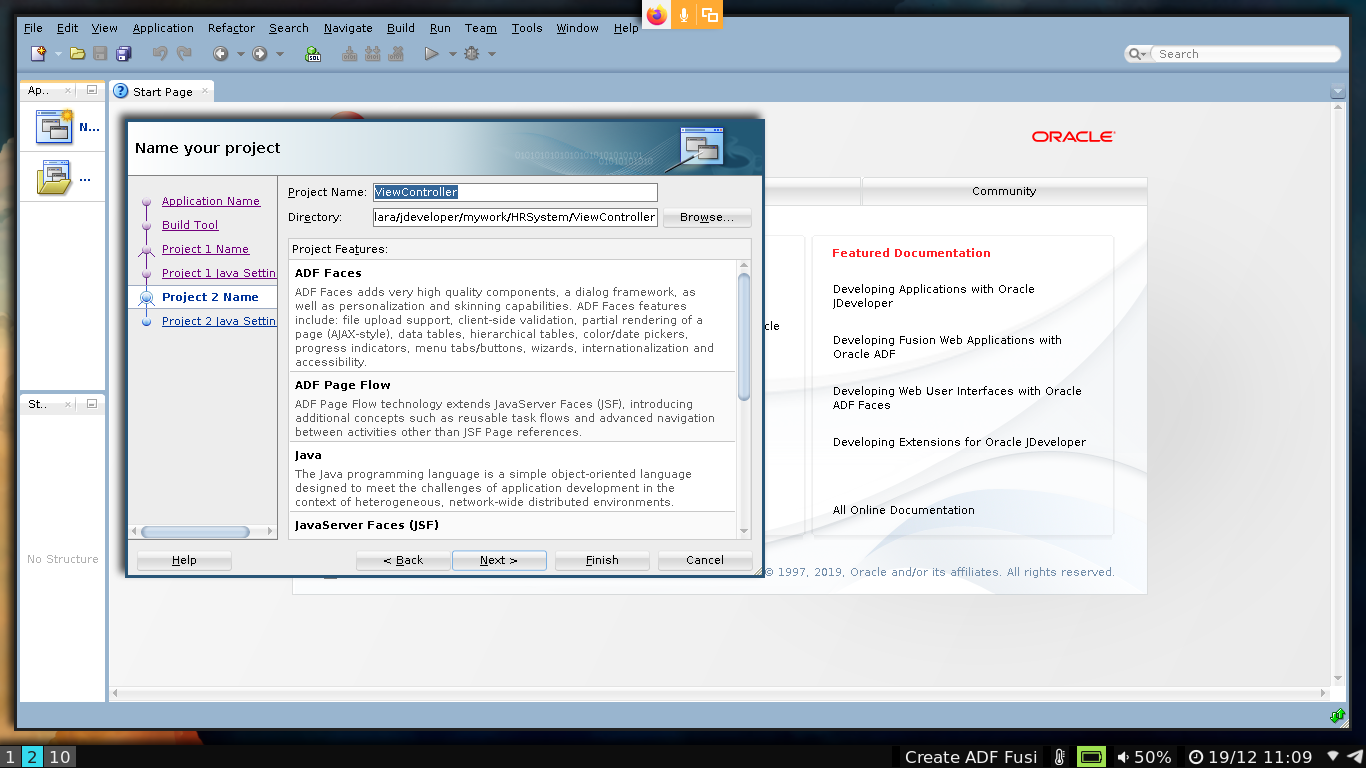
\includegraphics[scale=0.4]{5.png}
\end{figure}

\begin{figure}[!h]
  \centering
    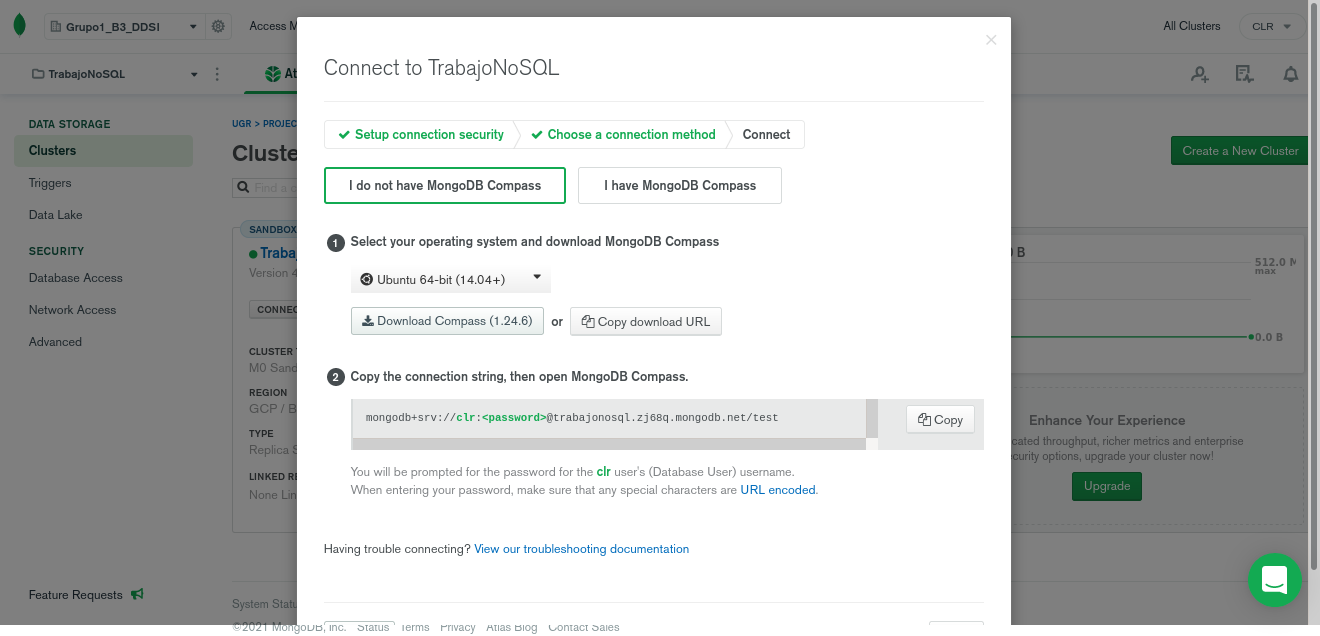
\includegraphics[scale=0.4]{6.png}
\end{figure}

\pagebreak
Descargamos Compass y introducimos la conexión que nos ha facilitado Atlas. Ya tenemos nuestra base de datos conectada al clúster de Atlas, y cualquier usuario que registremos desde Atlas a nuestro proyecto podrá conectarse al clúster desde Compass y trabajar en él.

\begin{figure}[!h]
  \centering
    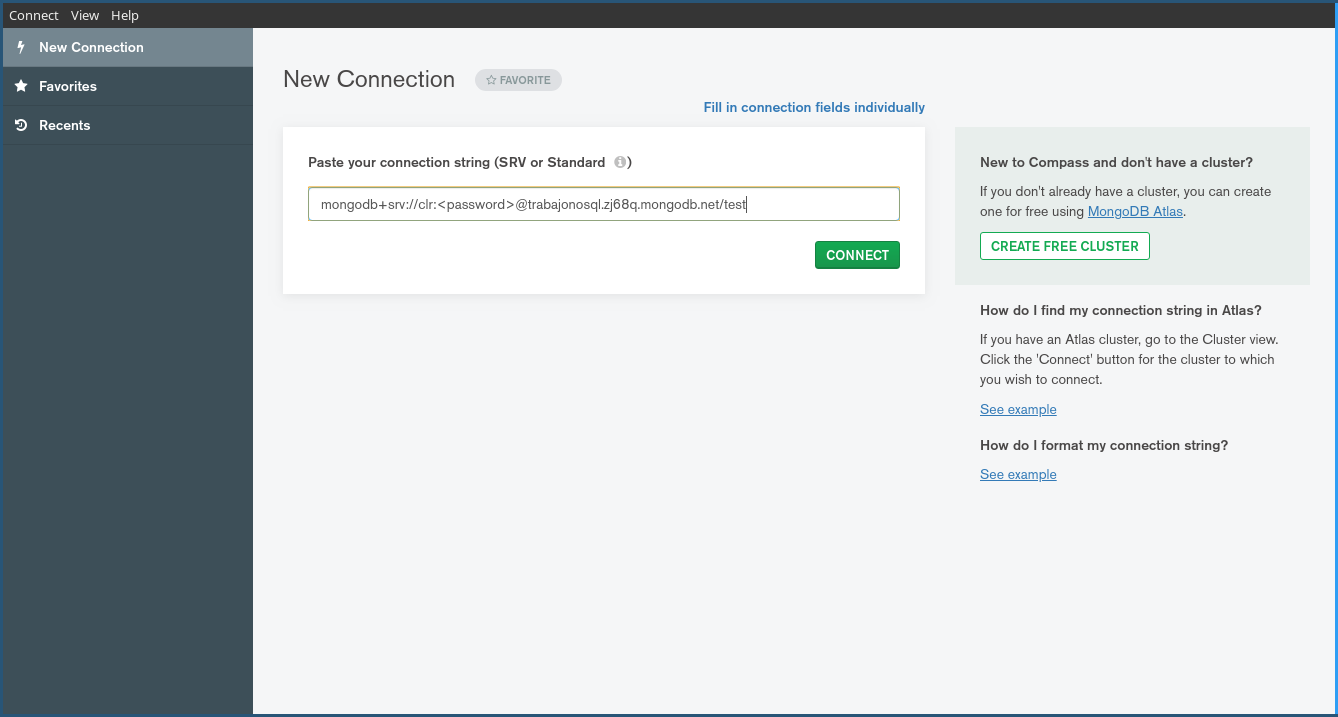
\includegraphics[scale=0.4]{7.png}
\end{figure}

\begin{figure}[!h]
  \centering
    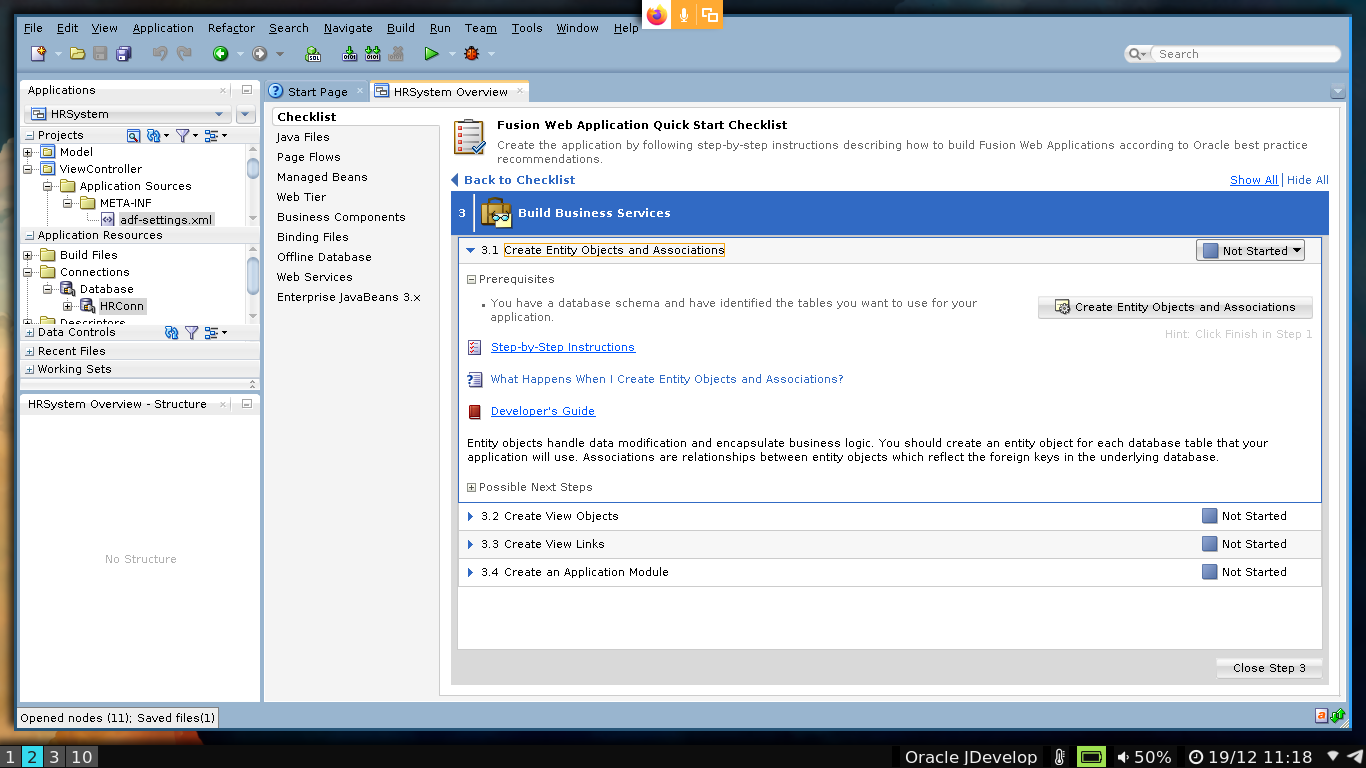
\includegraphics[scale=0.4]{8.png}
\end{figure}
